\chapter{Textos i formats}
\label{se:EPT}

\section{Documents de text}

El tipus de fitxer bàsic de treball del professional de la traducció
sol ser un fitxer amb text, és a dir, un text informatitzat, també
anomenat \emph{document de text}. Aquest fitxer pot contenir, a més
del text mateix, informació sobre la presentació: el format dels
paràgrafs i de les pàgines, sobre els tipus i les grandàries de lletra
que s'usen amb cada mot, etc., o sobre l'organització del contingut
(indicacions que una determinada part del text és un títol de capítol,
o una nota a peu de pàgina, etc.).  Un text informatitzat pot tenir
orígens diversos:
\begin{itemize}
\item Pot haver estat generat per un altre programa d'ordinador, per
  exemple a partir de les dades contingudes en alguna base de dades
  (vegeu el capítol.~\pageref{se:basesdades}).
\item El podem haver rebut annex a un missatge de correu electrònic
  (vegeu l'apartat~\ref{ss:correue} o per missatgeria instantània
  (vegeu l'apartat~\ref{ss:missinst}).
\item El podem haver descarregat (copiat) d'algun servidor d'Internet
  (vegeu la pàg.~\pageref{pg:ftp}).
\item El podem haver generat, potser a partir d'un altre
  text, usant un \emph{processador de textos} (vegeu
  l'apartat~\ref{ss:proctext}).
\item El pot haver generat un \emph{sistema de reconeixement de la
    parla} (vegeu la secció~\ref{ss:recparla}) a partir de la veu de
  la persona que l'ha dictat.
\item El pot haver generat un \emph{sistema de reconeixement de textos
    escrits} a partir d'un text tipografiat o manuscrit (vegeu la
  secció~\ref{ss:recautcar}).
\end{itemize}

%%%%%%%%%%%%%
\section{Formats de text}
\label{ss:formats}

\com{Caldria fer més èmfasi en els problemes que ocasionen els
  formats}

Un \emph{text informatitzat} és, com qualsevol porció de dades
informatitzada, una \emph{seqüència de bits}, és a dir, d'\emph{uns} i
\emph{zeros} de l'estil de la següent:

\begin{center}
 \texttt{010000010100110101001001\ldots}
\end{center}

Com ja hem vist en l'apartat~\ref{ss:memoria}, els \emph{bits} van
normalment en grups de vuit (\emph{bytes} o \emph{octets}):
\begin{center}
 \texttt{01000001 01001101 01001001\ldots}
\end{center}

Hi ha moltes maneres d'organitzar aquests octets per a emmagatzemar
els textos.  Molts dels problemes que apareixen quan es tracten textos
amb l'ordinador provenen de discrepàncies quant a la manera de fer-ho.
En les seccions següents estudiarem dos aspectes importants que
anomenarem \emph{codificació} i \emph{format} propiament dit.

La \emph{codificació} és l'assignació d'una seqüència concreta, d'un o més
\emph{octets}, a cada caràcter possible d'un text. Aquesta codificació consta de dues fases: en la
primera, s'assigna a cada caràcter un nombre enter positiu anomenat
\emph{punt de codi} o simplement \emph{codi}; per exemple:
``\texttt{a}'' $\to$ 97; ``\texttt{?}'' $\to$ 63, etc. En la segona
fase, anomenada de vegades \emph{serialització}, els codis es
converteixen en octets assignant-los una determinada seqüència de bits
(per exemple: 97 $\to$ \texttt{01100001}; 63 $\to$ \texttt{00111111}).


D'altra banda, els textos, a més de caràcters, contenen informació de
\emph{format}. Per això, és necessària l'assignació de \emph{codis} (que
també es convertiran en octets) per a regular altres característiques
del text:
\begin{itemize}
  \item l'aparença \emph{visual} o de
    presentació (per exemple, ``inici cursives'', ``final negretes'',
    ``lletra de 16 punts''), o
  \item l'\emph{estructura} (és a dir, l'organització del contingut,
    per exemple, ``títol de secció'', ``llista numerada'', ``nota a
    peu de pàgina'', ``fila d'una taula'', etc.)
\end{itemize}

\section{Codificació}

\subsection{L'ASCII original de 7 bits}

Com ja s'ha comentat en la pàgina~\pageref{pg:ASCII}, per a
emmagatzemar textos s'ha usat històricament el codi ASCII com a codi
bàsic. Aquest codi assigna un número de 7 bits a cada caràcter, de
manera que permet emmagatzemar un caràcter per octet i encara en sobra
un bit. La taula~\ref{tb:ASCII} mostra alguns exemples de codis
ASCII. Els codis ASCII del 0 al 31 no corresponen a caràcters
imprimibles sinó a \emph{caràcters de control} que tenen noms
especials i s'usen per a un control rudimentari del format i de la
transmissió dels textos.

\subsection{Extensions d'ASCII a 8 bits}
\label{s3:ISO}

ASCII no té codis per als caràcters especials que usen algunes
llengües europees com \texttt{ç}, \texttt{ä}, \texttt{ú}, etc.; amb
l'arribada dels microordinadors en els anys vuitanta es va decidir
ampliar el codi ASCII, de 7 bits i per tant amb $2^7=128$
possibilitats, a un codi de 8 bits amb $2^8=256$ possibilitats; el
vuité bit o ``bit 7''\footnote{Recordeu que en informàtica és comú
  comptar començant pel zero.}---el primer per l'esquerra--- és 1 per
als caràcters especials (numerats del 128 al 255) i zero per als
caràcters estàndards d'ASCII.  El fet que hi haja més d'una manera
estàndard d'usar els nous codis fa que de vegades els textos amb
caràcters especials no queden bé quan passem d'un processador de
textos (o un editor de textos) a un altre (els caràcters d'ASCII es
veuen normalment bé: els que fallen són els nous).  En la nostra àrea
geogràfica s'usa normalment la codificació ANSI Latin-1, també
coneguda com a ISO-8859-1 (vegeu la taula~\ref{tb:ISO88591}); aquesta
codificació serveix per a les llengües següents: \emph{afrikaans}
(llengua germànica parlada en la República de Sudàfrica), alemany,
anglés, basc, català, danés, escocés, espanyol, feroés, finés,
francés, gallec, irlandés, islandés, italià, neerlandés, noruec,
portugués i suec.\footnote{Recentment s'ha fet una modificació
  anomenada ISO-8859-15, per a incloure, entre altres, el símbol de
  l'euro i resoldre alguns problemes referents al francés i al finés.}
El sistema operatiu Windows de Microsoft usa la codificació de 8 bits
anomenada CP-1252, també anomenada \emph{WinLatin-1}, que és més
àmplia que ISO-8859-1 ja que usa alguns dels codis 128--159 per a
caràcters (per exemple, usa el codi 128 per al símbol de l'euro). Hi
ha altres codificacions en la família ISO-8859; per exemple,
l'albanés, el bosni, el croat, el txec, l'hongarés, o el romanés usen
una codificació anomenada ISO-8859-2 o \emph{Latin-2}, el letó, el
lituà i l'estonià usen l'ISO-8859-4 o \emph{Latin 4}, el rus usa
l'ISO-8859-5 que conté l'alfabet ciríl·lic a més de l'alfabet llatí
bàsic, etc. Per això, és molt important conéixer quin esquema de
codificació de caràcters s'ha usat en un document de text determinat
per a poder-lo llegir correctament; alguns formats de text inclouen
aquesta informació dins del mateix document.

Fixeu-vos que si en un document ISO-8859-1 s'escriu la frase \emph{Què
  és això?}, on els caràcters ``\texttt{è}'', ``\texttt{é}'' i
``\texttt{ò}'' tenen codis més alts (233, 232 i 242 respectivament), i
provem a llegir-lo com si fóra un document ISO-8859-2, llegirem
\emph{Quč és aixň?}, ja dos d'aquests codis (233 i 242) tenen una
altra interpretació en aquesta codificació (``\texttt{č}'' i
``\texttt{ň}'' respectivament).


\begin{table}
\begin{center}
\begin{tabular}{c|l|l}
\hline\hline \textsc{Codi binari} & \textsc{codi decimal} &
\textsc{caràcter} \\
\hline
\texttt{0000000} & 0 & NUL (caràcter nul)  \\
$\cdots$ & $\cdots$ & $\cdots$ \\
\texttt{0001001} & 9 & TAB (tabulador) \\
\texttt{0001010} & 10 & NL (nova línia) \\
$\cdots$ & $\cdots$ & $\cdots$ \\
\texttt{0001101} & 13 & CR (retorn del carro) \\
$\cdots$ & $\cdots$ & $\cdots$ \\
\texttt{0100000} & 32 & (un espai en blanc) \\
\texttt{0100001} & 33 & \texttt{!} \\
\texttt{0100010} & 34 & \verb+"+ \\
$\cdots$ & $\cdots$ & $\cdots$ \\
\texttt{0110000} & 48 & \texttt{0} \\
\texttt{0110001} & 49 & \texttt{1} \\
$\cdots$ & $\cdots$ & $\cdots$ \\
\texttt{0111000} & 56 & \texttt{8} \\
\texttt{0111001} & 57 & \texttt{9} \\
$\cdots$ & $\cdots$ & $\cdots$ \\
\texttt{1000000} & 64 & \texttt{@} \\
\texttt{1000001} & 65 & \texttt{A} \\
\texttt{1000010} & 66 & \texttt{B} \\
$\cdots$ & $\cdots$ & $\cdots$ \\
\texttt{1011010} & 90 & \texttt{Z} \\
\texttt{1011011} & 91 & \texttt{[} \\
$\cdots$ & $\cdots$ & $\cdots$ \\
\texttt{1100000} & 96 & \verb+`+ \\
\texttt{1100001} & 97 & \texttt{a} \\
\texttt{1100010} & 98 & \texttt{b} \\
$\cdots$ & $\cdots$ & $\cdots$ \\
\texttt{1111010} & 122 & \texttt{z} \\
\texttt{1111011} & 123 & \verb+{+ \\
$\cdots$ & $\cdots$ & $\cdots$ \\
\texttt{1111110} & 126 & \verb+~+ \\
\end{tabular}
\end{center}
\caption{Alguns exemples del codi ASCII. Els codis del 0 al 31 no
  corresponen a caràcters imprimibles sinó a caràcters de control.}
\label{tb:ASCII}
\end{table}

\begin{table}
\begin{center}
\begin{tabular}{c|l|l}
\hline\hline \textsc{Codi binari} & \textsc{codi decimal} &
\textsc{caràcter} \\
\hline
\texttt{10100000} & 160 & (espai no trencable)  \\
\texttt{10100001} & 161 & \texttt{¡} \\
$\cdots$          & $\cdots$ & $\cdots$ \\
\texttt{10110101} & 181 & $\mathtt{\mu}$ \\
\texttt{10110110} & 182 & \texttt{¶} \\
\texttt{10110111} & 183 & \texttt{·} \\
\texttt{10111000} & 184 & \texttt{¸} \\
$\cdots$          & $\cdots$ & $\cdots$ \\
\texttt{11000000} & 192 & \texttt{À} \\
\texttt{11000001} & 193 & \texttt{Á} \\
\texttt{11000010} & 194 & \texttt{Â} \\
\texttt{11000011} & 195 & \texttt{Ã} \\
\texttt{11000100} & 196 & \texttt{Ä} \\
\texttt{11000101} & 197 & \texttt{Å} \\
\texttt{11000110} & 198 & \texttt{Æ} \\
\texttt{11000111} & 199 & \texttt{Ç} \\
\texttt{11001000} & 200 & \texttt{È} \\
\texttt{11001001} & 201 & \texttt{É} \\
\texttt{11001010} & 202 & \texttt{Ê} \\
\texttt{11001011} & 203 & \texttt{Ë} \\
\texttt{11001100} & 204 & \texttt{Ì} \\
\texttt{11001101} & 205 & \texttt{Í} \\
\texttt{11001110} & 206 & \texttt{Î} \\
\texttt{11001111} & 207 & \texttt{Ï} \\
$\cdots$          & $\cdots$ & $\cdots$ \\
\texttt{11100000} & 224 & \texttt{à} \\
\texttt{11100001} & 225 & \texttt{á} \\
\texttt{11100010} & 226 & \texttt{â} \\
\texttt{11100011} & 227 & \texttt{ã} \\
\texttt{11100100} & 228 & \texttt{ä} \\
\texttt{11100101} & 229 & \texttt{å} \\
\texttt{11100110} & 230 & \texttt{æ} \\
$\cdots$          & $\cdots$ & $\cdots$ \\
\texttt{11111111} & 255 & \texttt{ÿ} \\

\end{tabular}
\end{center}
\caption{Alguns exemples d'ISO-8859-1. Els codis del 0 al 127 són com
  els d'ASCII. Els codis del 128 al 159 no estan assignats.}
\label{tb:ISO88591}
\end{table}

\subsection{Unicode}
% Millorar la descripció d'unicode mirant els man d'unicode i utf-8

Els codis de 8 bits com ANSI són adequats per a la major part de les
llengües europees, les quals es basen en l'alfabet llatí amb algunes
modificacions, però hi ha llengües al món que tenen sistemes
d'escriptura molt complexos amb milers de símbols diferents, com ara
el xinés o el japonés. Dues-centes cinquanta-sis combinacions no són
suficients per a aquestes llengües i s'hi han proposat diverses
solucions.  \emph{Unicode}\footnote{URI \url{http://www.unicode.org}}
(ISO 10646) és un nou estàndard per a fitxers de text que permet
codificar pràcticament totes les llengües del món i fins i tot mesclar
diversos alfabets en un mateix fitxer (Unicode té 31 bits; és a dir,
permet $2^{31}=2.147.483.648$ caràcters diferents). La versió més
comunament usada d'Unicode (BMP, \emph{Basic Multilingual Plane}) té
65534 caràcters; això comportaria l'ús de 2 octets (16 bits) en
comptes d'un ($2^{16}=65536$); això faria que un text Unicode senzill
fóra el doble de gran que el text ASCII corresponent, però hi ha
mètodes de serialització d'Unicode, com l'UTF-8, que en el cas de les
llengües europees amb alfabet llatí estalvia espai perquè usa un únic
octet per als codis ASCII (del 0 al 127, els més freqüents), i més
d'un octet per als codis següents (així, a més, és compatible amb
l'ASCII). En concret, UTF-8 usa
\begin{itemize}
\item per als codis del 0 al 127, 1 octet (compatible amb  ASCII)
\item per als codis del 128 al 2047, 2 octets
\item per als codis del 2048 al 65535, 3 octets, i així successivament.
\end{itemize}

\subsection{Limitacions}

Tot i que ampliem l'ASCII a ISO-8859 o Unicode, encara és molt
limitat.  Per exemple, si volem que un text tinga un cert format,
només podrem usar caràcters de control com ara l'espai en blanc, el
tabulador, el salt de línia, etc.  Per exemple, no podrem canviar
fàcilment de tipus o de grandària de lletra, o indicar que una
determinada part del text és el títol d'una secció o el text d'una
nota a peu de pàgina. De qualsevol manera, ASCII i les codificacions
ISO-8859-$X$, o Unicode, encara s'usen en aplicacions com ara el
correu electrònic, o quan volem que un text ---el contingut del qual
és molt més important que l'aparença--- puga ser llegit per qualsevol
usuari sense importar el processador de textos que use; els textos
d'aquesta mena s'anomenen de vegades \emph{textos plans} i
s'emmagatzemen normalment en fitxers amb noms que tenen l'extensió
\texttt{.txt}.  Aquests textos es poden produir i llegir amb qualsevol
\emph{editor de textos} (vegeu l'epígraf~\ref{ss:proctext}).


\section{Format pròpiament dit}

Els documents de text són en general més rics que simples seqüències
de caràcters. Necessitem codificar-hi informació estructural (sobre
l'organització del contingut del document) o presentacional (sobre
l'aparença que tindrà quan es presente): tipus i grandàries de lletra,
format dels paràgrafs, notes a peu de pàgina, etc. Per a guardar
aquesta informació, s'usen:
\begin{itemize}
\item D'una banda, codificacions o formats basats en text
  (ISO-8859-$X$, Unicode, etc.) com ara SGML (\emph{standardized
    generalized markup language}), la seua versió simplificada (i molt
  més estesa) XML (\emph{extensible markup language}), el tipus SGML
  anomenat HTML (\emph{hypertext markup language}), el format proposat
  per Microsoft anomenat RTF (\emph{rich text format}, no relacionat
  amb SGML), o el llenguatge per a impressores anomenat
  Postscript. Tots aquests formats usen combinacions
  especials\footnote{i poc freqüents en textos usuals} de caràcters de
  text per a indicar aquestes característiques d'estructuració o de
  presentació.\footnote{Aquests caràcters que indiquen el format no són
    normalment visibles per a la persona usuària mentre redacta o
    veu el document, excepte si demana explícitament que els vol
    veure.} 
\item D'altra banda, hi ha els formats particulars dels processadors
  de textos comercials com ara Corel WordPerfect o Microsoft Word, que
  usen esquemes diferents, basats en codis binaris no relacionats amb
  l'ASCII.\footnote{Hi ha una tendència a considerar el format de
    document de Microsoft Word, amb extensió \texttt{.doc}, com la
    manera estàndard d'enviar documents de text annexos a un missatge
    electrònic, sense considerar el fet que aquest format és privat i
    està associat a l'ús d'un determinat producte no lliure i de codi
    font tancat. El format \texttt{.docx} també anomenat Office Open
    XML o OOXML, està millor documentat i estandarditzat i pot ser
    processat més satisfactòriament amb processadors lliures i de codi
    font obert.}
\end{itemize}
Com ja s'ha dit, l'ús de formats de text més avançats no només serveix
per a determinar-ne la presentació en la pantalla o quan són impresos;
com veurem més avall, en el cas de SGML i XML, el format serveix per a
\emph{estructurar} el document de text en unitats directament
relacionades amb el contingut del document, com ara seccions, títols
de secció, llistes, paràgrafs, etc.; aquesta estructuració interna del
document pot ser usada després per a fer recerques d'informació amb
l'ajuda de l'estructura definida, com ara buscar un mot concret només
en títols de secció, o també per a produir-ne una presentació concreta
del document, com veurem més endavant. De fet, recentment, amb
l'aparició de XML (vegeu l'apartat~\ref{s3:XML}), s'observa una tendència cap a
l'adopció de formats de document estructurats, és a dir, no
relacionats únicament amb la presentació, sinó també amb l'estructura
pròpia del document, formats normalment concebuts de manera que la
presentació desitjada es puga produir a partir de l'estructura usant
fitxers (anomenats \emph{fulls d'estil}) amb regles d'estil ben
definides (vegeu la secció~\ref{ss:separac}).

\section{SGML i XML}
%\subsection{SGML i XML}
\label{s3:SGML}
\label{ss:SGML}

\subsection{SGML}

SGML, el llenguatge estàndar generalitzat de marques, havia tingut un
èxit relatiu fins a mitjans dels noranta; però l'aparició cap a finals
dels noranta d'una versió restringida i simplificada de SGML anomenada
XML ha impulsat enormement l'adopció dels formats d'estructuració de
documents, de tal manera que en l'actualitat s'usa XML moltíssim més
que el SGML original; per això, ens centrarem en aquest últim
format. De tota manera, encara hi ha formats molt importants que es
basen en SGML, com el llenguatge de marques per a hipertextos HTML (vegeu l'apartat~\ref{s3:HTML})
(excepte pel més recent, HTML5, estandarditzat el 2014, que ja no és
una aplicació SGML). Hi ha també versions estàndards de HTML conegudes
com XHTML, que es basen directament en XML (vegeu l'apartat~\ref{s3:XML}).\footnote{Noteu que
  HTML5 també té una versió \emph{serialitzada en XML}, XHTML4}

\subsection{XML}
\label{s3:XML}

\subsubsection{Marques}

Un document XML és un document de text on, a més del text pròpiament
dit, podem trobar \emph{etiquetes} o \emph{marques} (en anglés
\emph{tags}) que donen informació sobre la naturalesa i l'organització
de cada un dels continguts del document; com ja s'ha dit, un document
XML és un document \emph{estructurat}. Per exemple, un document XML
corresponent a un FAX\todo{Per discutir: canviar el document de FAX per un altre que tinga més sentit.} podria tenir l'aparença que es mostra en la
figura~\ref{fg:faxXML}.  La primera línia declara que el document és
un document XML de la versió 1.0 i que el joc de caràcters que usa és
l'ISO-8859-1 (o ``Latin 1''), vegeu l'apartat~\ref{s3:ISO}. Com s'hi pot veure, les etiquetes que
apareixen entre parèntesis angulars indiquen les diverses parts del
document, anomenades \emph{elements}.  Típicament, s'obrin amb
\texttt{<}\emph{nom}\texttt{>} i es tanquen amb
\texttt{</}\emph{nom}\texttt{>}.  En l'exemple, es pot veure que un
fax (\texttt{<FAX>}\ldots\texttt{</FAX>}) té un destinatari, un
remitent, una data i un text; és a dir, els elements poden contenir
altres elements; les marques funcionen com a parèntesis. Seguint amb
la jerarquia d'inclusió d'elements en altres, tant el destinatari com
el remitent tenen nom i número, i el text es compon de paràgrafs
(\texttt{<P>}\ldots\texttt{</P>}).

\com{No sé si convindria canviar l'exemple del fax per un altre de més
  adequat...}

\subsubsection{Documents XML ben formats}

Aquestes són algunes de les característiques que fan que un document
XML estiga \emph{ben format}, és a dir, siga un document XML i no una
altra cosa:
\begin{itemize}
\item Cada etiqueta d'inici d'element de la forma
  \texttt{<}\emph{nom}\texttt{>}, \texttt{<}\emph{nom}
  \emph{atribut}\texttt{=}\emph{valor} \texttt{>},
  \texttt{<}\emph{nom} \emph{atribut}\texttt{=}\emph{valor}
  \emph{atribut}\texttt{=}\emph{valor} \texttt{>}, etc. (amb zero o
  més assignacions de valors a atributs) ha d'estar emparellat amb una
  etiqueta de final d'element de la forma
  \texttt{</}\emph{nom}\texttt{>}, sense atributs però amb el mateix
  nom.\footnote{En SGML es permet que alguns elements es tanquen
    \emph{implícitament}, sense necessitat d'una etiqueta de final
    d'element.} Si l'element és buit,
  \texttt{<}\emph{nom}\ldots\texttt{></}\emph{nom}\texttt{>}, també es
  pot escriure \texttt{<}\emph{nom}\ldots\texttt{/>}
\item Un element pot contenir qualsevol nombre d'elements.
\item Els elements no es poden solapar o creuar: no és possible
  escriure, per exemple, \texttt{<a>text<b>més text</a>més text encara
    </b>}.
\item El document conté un únic element \emph{arrel} que conté tots
  els elements del text.
\item El document pot contenir comentaris entre \texttt{<!--} i
  \texttt{-->} o instruccions de processament del tipus
  \texttt{<?}\emph{nom}\ldots\texttt{?>} en qualsevol lloc excepte dins
  de les etiquetes.
\item Els valors dels atributs han d'anar entre cometes dobles
  (\texttt{"}\emph{valor}\texttt{"}) o simples
  (\texttt{'}\emph{valor}\texttt{'}).
\item Un element no pot tenir dos atributs amb el mateix nom.
\item Els caràcters \texttt{<} i \texttt{\&} no poden aparéixer en el
  text dels elements ni dels atributs. Això és perquè \texttt{<}
  indica el començament d'une etiqueta i \texttt{\&} el començament
  d'una \emph{entitat} com ara \texttt{\&copy;} que es pot usar per a
  representar el càracter \emph{©}: si es necessiten aquests caràcters
  s'han d'escriure \texttt{\&lt;} i \texttt{\&amp;}.  
\end{itemize}
Com es pot veure, aquestes regles que defineixen un document XML ben
format no diuen quines etiquetes són vàlides i quines no, o quins
atributs pot tenir un determinat element, o quins elements poden anar
dins de un determinat element, en quin ordre o en quina
quantitat. 

\subsubsection{Tipus de documents}

\com{No sé si l'exemple del FAX és adequat}

Per a especificar, per a un tipus determinat de document XML, quines
etiquetes són vàlides, quins atributs pot tenir cada element, o quins
elements poden anar dins d'un determinat element, en quin ordre o en
quina quantitat, es pot usar una DTD (\emph{document type definition} o
definició del tipus de document).\footnote{Les DTD no són l'única manera d'especificar
    famílies de documents XML; una altra manera més potent són els
    anomenats \emph{esquemes XML} (anglés \emph{XML schema}).} 
\todo{Hauríem de posar el material sobre validació de les pràctiques ací?}

La segona línia del fax de la figura~\ref{fg:faxXML} especifica el
tipus del document tot indicant d'una banda l'etiqueta arrel o
principal del document (\texttt{FAX}) i l'URI (\texttt{SYSTEM}) on es
troba la DTD. Aquesta DTD es veu en la figura~\ref{fg:faxDTD};
examinem ara la DTD línia a línia per a comprendre com s'usen les DTD per
a definir famílies (tipus) de documents en XML:
\begin{enumerate}
\item La primera línia declara que la DTD és una DTD de la versió
1.0 i que el joc de caràcters que s'usa és l'ISO-8859-1, també
conegut com a Latin-1.
\begin{small}\begin{verbatim}
<?xml version="1.0" encoding="ISO-8859-1"?>
\end{verbatim}\end{small}
\item La segona línia és un comentari. Els comentaris comencen amb
  \verb+<!--+ i acaben amb \verb+-->+ i es poden situar en qualsevol
  part d'una DTD.
\begin{small}\begin{verbatim}
<!-- Aquest és l'exemple de DTD de FAX -->
\end{verbatim}\end{small}
\item Les línies següents defineixen l'estructura del document
  definint els seus \emph{elements}. La línia
\begin{small}\begin{verbatim}
<!ELEMENT FAX (DESTINATARI, REMITENT?, DATA, TEXT)>
\end{verbatim}\end{small}
defineix l'element arrel o principal, \texttt{FAX}, i especifica que
es compon (en l'ordre especificat) d'un \texttt{DESTINATARI}, un
\texttt{REMITENT} opcional (indicat amb \texttt{?}), d'una \texttt{DATA} i d'un
\texttt{TEXT}. 
\item El \texttt{DESTINATARI} del fax té dues parts: el \texttt{NOM}
  (opcional) i el número (\texttt{NUM}).
\begin{small}\begin{verbatim}
<!ELEMENT DESTINATARI (NOM?, NUM)>
\end{verbatim}\end{small}
\item El remitent es defineix igual:
\begin{small}\begin{verbatim}
<!ELEMENT REMITENT (NOM?, NUM)>
\end{verbatim}\end{small}
\item El \texttt{NOM}, el número \texttt{NUM} i la \texttt{DATA}
  contenen text sense marques (indicat amb \verb+#PCDATA+).
\begin{small}\begin{verbatim}
<!ELEMENT NOM (#PCDATA)>
<!ELEMENT NUM (#PCDATA)>
<!ELEMENT DATA (#PCDATA)>
\end{verbatim}\end{small}
\item El \texttt{TEXT} es compon d'un o més (\texttt{+}) paràgrafs
  (\texttt{P}). Si volguérem que el text estiguera compost per \emph{zero} o
  més paràgrafs usaríem ``\texttt{*}'' en comptes de ``\texttt{+}''.
\begin{small}\begin{verbatim}
<!ELEMENT TEXT (P)+>
\end{verbatim}\end{small}
\item Finalment, els paràgrafs contenen text.
\begin{small}\begin{verbatim}
<!ELEMENT P (#PCDATA)>
\end{verbatim}\end{small}
\end{enumerate}
Una de les aplicacions més importants de les DTD és que serveixen per a la
validació automàtica dels documents: un programa \emph{validador} llegeix la
DTD i el document XML i decideix si aquest últim és vàlid, és a dir, si segueix
l'especificació donada en la DTD
De fet, el \emph{significat} de les etiquetes (és
a dir, quines conseqüències tindran quan es processe el document XML) l'ha
d'establir el programa o els programes que processaran els documents. 
(i les DTD poden servir també per a assegurar que els documents processats són vàlids).
Com ja
s'ha dit, el significat de les etiquetes pot estar associat, per exemple, a la
manera (\emph{estil}, vegeu la p.~\pageref{pg:estil}) de presentar el document
quan s'imprimeix (per exemple, el destinatari del fax pot anar en negretes),
però també podria servir per a facilitar el processament de la informació (per
exemple, buscar tots els faxos que tenen un determinat destinatari,\todo{cal canviar-ho si canviem l'exemple} o, en
llibres codificats en XML, decidir quines parts han de ser traduïdes
automàticament de l'espanyol a l'anglés i quines no perquè són cites
literàries.\footnote{Hi ha un estàndard anomenat TEI, de l'anglés \emph{text encoding initiative}, ``iniciativa de codificació de textos'' (\url{http://www.tei-c.org}) que usa famílies de DTD per a definir diferents tipus d'obres (literàries i no literàries). De fet, existeixen, d'una banda, les antigues DTD  per a SGML, i, d'altra, les DTD TEI per a XML.}
  \todo{Introduïm TEI ací com a exemple d'aplicació XML??} Fins i tot fitxers que normalment no
consideraríem documents, com ara les memòries de traducció (vegeu el
capítol~\ref{se:memtrad}) s'estructuren de manera estàndard usant un format
basat en XML anomenat TMX.  \com{L'últim paràgraf es pot millorar}


  Una altra aplicació de les DTD és fer-les servir per a facilitar
  l'edició de documents XML vàlids: un editor de documents XML pot
  consultar la DTD per suggerir a la persona usuària l'element o
  elements correctes en el context actual, o per emetre un missatge
  d'error tan aviat com el document perda la seua validesa.


\begin{figure}
\begin{center}
\begin{verbatim}
<?xml version="1.0" encoding="ISO-8859-1"?>
<!DOCTYPE FAX SYSTEM "http://www.dlsi.ua.es/%7Emlf/iat/fax.dtd">
<FAX>
<DESTINATARI>
       <NOM>Mikel L. Forcada</NOM>
       <NUM>+34-96-590-9326</NUM>
</DESTINATARI>
<REMITENT>
       <NOM>Letícia Ibaizábal</NOM>
       <NUM>+34-96-999-9999</NUM>
</REMITENT>
<DATA>23 de setembre de 2000</DATA>
<TEXT>
<P>Mikel, m'agradaria que m'enviares el text de l'última
pràctica d'IAT.</P>
<P>Ah, i també; l'examen de febrer. Gràcies.</P>
</TEXT>
</FAX>
\end{verbatim}
\end{center}
\caption{Un FAX en XML}
\label{fg:faxXML}
\end{figure}

\begin{figure}
\begin{center}
\begin{verbatim}
<?xml version="1.0" encoding="ISO-8859-1"?>
<!-- Aquest és l'exemple de DTD de FAX -->
<!ELEMENT FAX (DESTINATARI, REMITENT?, DATA, TEXT)>
<!ELEMENT DESTINATARI (NOM?, NUM)>
<!ELEMENT REMITENT (NOM?, NUM)>
<!ELEMENT NOM (#PCDATA)>
<!ELEMENT NUM (#PCDATA)>
<!ELEMENT DATA (#PCDATA)>
<!ELEMENT TEXT (P)+>
<!ELEMENT P (#PCDATA)>
\end{verbatim}
\end{center}
\caption{La DTD que defineix els faxos com el de la fig.~\ref{fg:faxXML}.}
\label{fg:faxDTD}
\end{figure}

\subsection{HTML}
\label{s3:HTML}

\com{Potser hi ha material sobre HTML del laboratori que es podria
  incloure ací per a completar la informació sobre com està
  estructurat un document HTML}

El format HTML (\emph{hypertext markup language} o \emph{llenguatge de
  marques per a hipertextos}) és un dels tipus de document que es
poden definir amb SGML (però no exactament amb XML; la versió XML de
HTML s'anomena XHTML\footnote{Definit en
  \url{http://www.w3.org/TR/xhtml1/}.}); HTML és molt important perquè
és el llenguatge en el que estan escrits els hipertextos d'Internet
(vegeu el capítol~\ref{se:Internet}) i el que interpreten els
navegadors (vegeu l'apartat~\ref{ss:navegadors}). En HTML, les marques
tenen un significat determinat. Originalment, les marques estaven
pensades per a expressar l'estructura del document, però amb el pas
del temps el significat de les marques ha canviat i actualment algunes
estan més aïna associades a la presentació del document durant la
navegació (tot i que, darrerament, sembla que a poc a poc es va
tornant al plantejament original amb iniciatives com ara XHTML, una
versió compatible amb XML del llenguatge HTML). Per exemple, HTML
indica el començament d'un segment de text destacat (emfatitzat) amb la marca
``{\tt <em>}'' (4 caràcters ASCII) i el final amb la marca ``{\tt
  </em>}'' (5 caràcters). HTML serveix per a codificar hipertextos:
els enllaços (hiperreferències) a altres documents (que al seu torn
poden també ser hipertextos) comencen amb ``\texttt{<a href="}
$\mathit{URI}$ \texttt{"}\texttt{>}'' ---on $\mathit{URI}$ és el
identificador del document enllaçat--- i acaben amb ``\texttt{</a>}'',
etc. Els documents HTML comencen idealment amb la marca
``\texttt{<html>}'' i acaben amb la marca ``\texttt{</html>}'', i
tenen, entre altres elements, un títol
(``\texttt{<title>}\ldots\texttt{</title>}'') i un cos
(``\texttt{<body>}\ldots\texttt{</body>}'').  Per exemple, el document
HTML que es mostra en la figura~\ref{fg:HTML} es mostraria en un
navegador aproximadament com en la figura~\ref{fg:HTMLnav}. Com es pot
veure, la primera línia, que comença amb ``\texttt{<!DOCTYPE}''
declara que el document és un tipus de document HTML estàndard segons
la versió 4.01 \emph{estricta} de HTML (hi ha diverses versions).  En
la tercera línia, l'etiqueta ``\texttt{<html>}'' indica el començament
del document XHTML, i l'etiqueta ``\texttt{</html>}'' del final indica
el final del document. Dins de l'element \texttt{html} trobem dos
elements: \texttt{head} (l'\emph{encapçalament}) i \texttt{body} (el
\emph{cos} del document).  Dins de l'encapçalament, un element
\texttt{meta} que no té contingut (fixeu-vos com s'obri i es tanca al
mateix temps) indica, a través de dues assignacions del tipus
\emph{atribut}\texttt{="}\emph{valor}\texttt{"}, que el \emph{joc de
  caràcters} que usa el document és l'ISO-8859-1, el més comú a Europa
occidental.\footnote{Per a escriure documents en \emph{txec} o en
  \emph{coreà}, caldria canviar part del valor de l'atribut
  \texttt{content} perquè la codificació ISO-8859-1 no permet escriure
  en aquests idiomes.} Dins de \texttt{head} també trobem l'element
\texttt{title}, el qual conté un títol que es presentarà, quan obriu
el document amb un navegador, en la barra del navegador, \emph{però no
  com a part del text del document}. Dins de \texttt{body} veiem
encapçalaments de nivell 1 (\texttt{h1}), encapçalaments de nivell 2
(\texttt{h2}), paràgrafs (\texttt{p}), parts del text destacades
(\texttt{em}), i enllaços (\texttt{a}). La taula~\ref{tb:15etiq} descriu algunes de les etiquetes més importants que s'usen en HTML.

\begin{figure}
\begin{center}
\begin{verbatim}
<!DOCTYPE HTML PUBLIC "-//W3C//DTD HTML 4.01 Strict//EN"
               "http://www.w3.org/TR/html4/strict.dtd">
<html>
  <head>
    <meta http-equiv="Content-Type"
          content="text/html; charset=iso-8859-1">
    <title>Títol del document</title>
  </head>

  <body>

    <h1>Encapçalament de nivell 1</h1>

    <h2>Encapçalament de nivell 2</h2>

    <p>Aquest és el <em>primer</em> paràgraf 
    d'aquest document. El navegador decideix com dividir-lo 
    en línies per a presentar-lo. Idealment, hauria 
    d'acabar amb una marca de final de paràgraf. </p>

    <h2>Un altre encapçalament de nivell 2</h2>

    <p>Aquest és l'<em>últim</em> paràgraf 
    d'aquest document HTML. Els documents HTML poden contenir 
    <a href="http://www.internostrum.com">enllaços</a> 
    a altres documents HTML, locals o remots. </p>

  </body>
</html>
\end{verbatim}
\end{center}
\caption{Un document HTML, tal com el presentaria un editor normal de
  textos o usant l'opció ``view HTML source'' (veure font HTML) del
  navegador. 
  %En aquest document HTML  no s'ha especificat el joc de
  %caràcters que s'usarà i per això els caràcters especials com ara les
  %lletres accentuades apareixen representades per \emph{entitats} que
  %comencen amb ``\texttt{\&}'' i acaben amb ``\texttt{;}''.
  }
\label{fg:HTML}
\end{figure}

\begin{figure}
\begin{center}
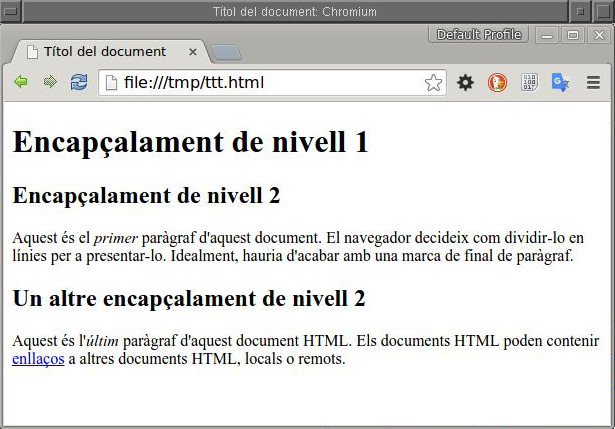
\includegraphics[scale=0.5]{vista-chromium.jpg}
  \end{center}
\caption{El document HTML de la figura~\protect\ref{fg:HTML}, vist a
  través d'un navegador determinat.}
\label{fg:HTMLnav}

\end{figure}

% \begin{figure}
% \begin{center}
% \framebox{\parbox{10cm}{\textsf{Títol del document
% }}}
% \framebox{\parbox{10cm}{
% \noindent{\bf\large Encapçalament de nivell 1}\vspace{1ex}

% \noindent{\bf Encapçalament de nivell 2}\vspace{1ex}

% \noindent\raggedright Aquest és el \textit{primer} paràgraf d'aquest document. El
% navegador decideix com dividir-lo en línies per a
% presentar-lo. Idealment, hauria d'acabar amb una marca de final de
% paràgraf.\vspace{1ex}

% \noindent{\bf Un altre encapçalament de nivell 2}\vspace{1ex}

% \noindent\raggedright Aquest és  l'\textit{últim}  paràgraf d'aquest document
% HTML. Els documents HTML poden contenir \underline{enllaços} a altres
% documents HTML, locals o remots. 

% }
% }
% \end{center}
% \caption{El document HTML de la figura~\protect\ref{fg:HTML}, vist a
%   través d'un navegador determinat.}
% \label{fg:HTMLnav}
% \end{figure}


\begin{table}
\caption{Alguns elements bàsics d'XHTML, la versió XML de HTML.}
\begin{center}
\begin{tabular}{l|l|p{5.5cm}}
  \hline\hline
  \textsf{Element} & \textsf{Descripció} & \textsf{Més informació} \\
  \hline
  \texttt{<html>}\ldots\texttt{</html>} & Conté tot el document & \\
  \hline
  \texttt{<head>}\ldots\texttt{</head>} & Encapçalament & \\\hline
  \texttt{<body>}\ldots\texttt{</body>} & Cos & \\\hline
  \texttt{<meta}\ldots\texttt{/>} & Informació sobre el document & L'element és
  buit \\\hline
  \texttt{<title>}\ldots\texttt{</title>} & Conté el títol del document & \\\hline
  \texttt{<br/>} & Salt de línia forçat & L'element és buit. \\\hline
  \texttt{<h1>}\ldots\texttt{</h1>} & Encapçalament de nivell 1 & \\\hline
  \texttt{<h2>}\ldots\texttt{</h2>} & Encapçalament de nivell 2 & \\\hline
  \(\cdots\) & \(\cdots\) & \(\cdots\) \\\hline
  \texttt{<h6>}\ldots\texttt{</h6>} & Encapçalament de nivell 6 & \\\hline
  \texttt{<p>}\ldots\texttt{</p>} & Paràgraf & 
  \\\hline
  \texttt{<ul>}\ldots\texttt{</ul>} & Llista sense numerar & Conté elements \texttt{li} \\\hline
  \texttt{<ol>}\ldots\texttt{</ol>} & Llista numerada & Conté elements \texttt{li} \\\hline
  \texttt{<li>}\ldots\texttt{</li>} & Element de llista & Pot contenir una altra
  llista en el seu interior. 
\\\hline
  \texttt{<em>}\ldots\texttt{</em>} & Èmfasi & \\\hline
  \texttt{<strong>}\ldots\texttt{</strong>} & Èmfasi fort & \\\hline
  \texttt{<code>}\ldots\texttt{</code>} & Exemple de codi & \\\hline
  \texttt{<a}\ldots\texttt{>}\ldots\texttt{</a>} & ``Àncora'' & Si porta un atribut
  \texttt{href="}URI\texttt{"}, el text entre ``\texttt{<a}\ldots\texttt{>}'' i
  ``\texttt{</a>}'' funciona com un enllaç al document que hi ha en l'URI.\\\hline
  \texttt{<img}\ldots\texttt{/>} & Imatge & L'atribut  \texttt{src="}URI\texttt{"} indica l'adreça on és la imatge. 
  L'atribut \texttt{alt="}\emph{text}\texttt{"} descriu la imatge amb paraules. L'element és buit.\\\hline
\end{tabular}
\end{center}
\end{table}

Quan estem mirant un document HTML amb un navegador, podem veure les etiquetes HTML que el formaten si seleccionem l'opció ``veure font
HTML'' (``view HTML source'') o similar que hi ha normalment en el
menú ``veure'' (``view'').

\subsection{RTF}
\label{s3:RTF}

RTF (\emph{rich text format}, és a dir, \emph{format de text ric}) va ser 
un format impulsat per l'empresa Microsoft per a facilitar
l'intercanvi de documents entre processadors de textos mantenint-ne el
format, i que encara s'usa de vegades. RTF també té etiquetes, les quals comencen normalment per una
barra invertida (\verb+\+); però els àmbits d'acció de les etiquetes
estan delimitats per claus (``\verb+{+\ldots\verb+}+'') en comptes de
per parelles d'etiquetes; per exemple, un segment en negretes s'indica
amb ``\verb+{\b+\ldots\verb+}+'', mentre que en HTML s'usa
``\verb+<B>+\ldots\verb+</B>+''. La figura~\ref{fg:RTF} mostra part
d'un document RTF, en la qual es veuen algunes comandes de
l'encapçalament (començant amb ``\verb+{\rtf1+...'') i on també
  s'observa la manera especial com es codifiquen alguns caràcters.

\begin{figure}
\begin{center}
\begin{verbatim}
{\rtf1\ansi\ansicpg1252
\end{verbatim}
[\ldots]
\begin{verbatim}
\par
{\b T\`edtol en negretes}\par
Text del par\`a0graf en lletra normal amb alguns incisos 
{\i en cursives} i una marca de final de par\`a0graf al 
final.\par  
Els car\`a0cters que no pertanyen a l'ASCII est\`a0ndard 
s'indiquen amb codis especials (en aquest cas s'ha usat 
ANSI, amb {\i codepage} 1252, com es veu al principi del 
document), com per exemple en el mot 
{\i ling\'fc\'edstica}.\par
\end{verbatim}
[\ldots]
\end{center}
\caption{Part d'un document de text en format RTF}
\label{fg:RTF}
\end{figure}


\subsection{PDF}\todo{Abans del PDF, afegir ODF i OOXML?}

PDF (de l'anglés \emph{portable document format}, format portable de
document) és un altre format desenvolupat per a capturar completament
les característiques presentacionals dels documents. En PDF, el
document es mostra exactament amb la mateixa aparença independentment
de l'ordinador, sistema operatiu o aplicació que fem servir per
veure'l. Els documents PDF poden emmagatzemar, a banda del text, tipus
de lletra, gràfics, sons, etc. Aquest format va ser impulsat en els
anys noranta per l'empresa Adobe, que ofereix en l'actualitat un
programa gratuït\footnote{però no lliure ni de codi font obert}
anomenat Adobe Acrobat Reader DC--- per visualitzar els
documents;\footnote{Hi ha alternatives lliures i de codi font obert
  com ara Sumatra PDF, Evince, Okular, etc. Fins i tot, els mateixos
  navegadors vénen ja amb visors de PDF.}  per crear-los podem usar
programes especialitzats o qualsevol processador de textos que permeta
\emph{exportar} (realment \emph{imprimir}) el nostre document a PDF.

\section{Processadors de textos}
\label{ss:proctext}

Un \emph{processador de textos} és un programa que permet crear i
modificar documents de text informatitzats. També s'hi poden usar {\em
  editors}: la diferència entre un processador de textos i un {\em
  editor} és que aquest últim programa és un processador de textos
plans (sense informació de format, etc.) que normalment s'usa per a
preparar textos en algun llenguatge artificial (per exemple, programes
escrits en algun llenguatge de programació) que serviran de entrada
per a un altre programa, o textos molt senzills on el format no és
crucial, com un missatge electrònic senzill.

El processament de textos també s'anomena \emph{tractament de
  textos} (paral$\cdot$le\-la\-ment al francés, \emph{traitement
  textes}). En anglés, l'èmfasi és sobre les paraules:
\emph{word processing}.

Per descomptat, aquesta secció no pretén instruir en l'ús de cap
processador de textos concret, sinó que vol descriure breument algunes
característiques comunes als processadors de textos que s'usen en
l'actualitat. De fet, l'ús dels processadors de text s'aprén molt
millor en el laboratori; a més, en vista del fet que els processadors
de textos canvien constantment, potser és millor no aprendre a usar un
processador concret sinó a buscar en cada processador les eines que
necessitem. Això és possible perquè la major part dels processadors
van fornits de manuals o de sistemes d'ajuda en línia; alguns tenen
fins i tot ``assistents'' que observen el que fa la persona usuària i
li suggereixen ---amb més o menys fortuna--- possibles accions en cada
moment.

Quant a l'\emph{aparença} del programa, la major part dels
processadors de text es manifesten bàsicament com una o diverses
finestres, cada una de les quals mostra una secció d'algun dels
documents de text informatitzats que estem creant i modificant (els
documents que tenim \emph{oberts}).  La tendència actual afavoreix que
el text es mostre tan paregut com siga possible a la versió impresa
que se'n produirà, quant a format, tipus de lletra, etc.\ (en anglés,
aquest concepte de fidelitat visual es resumeix amb el mot {\em
  wysiwyg}, fet amb les sigles de ``what you see is what you get'', és
a dir, ``el que veieu és el que obtindreu''); la
secció~\ref{s3:problema_wysiwyg} descriu alguns problemes derivats
d'aquesta tendència.

Quant a l'\emph{operació}, els processadors de text assumeixen que la major
part dels caràcters que teclegem s'han d'inserir darrere del caràcter
que actualment es troba destacat amb una marca anomenada {\em
  cursor} de text (pot ser diferent del cursor o apuntador que indica
la posició virtual del ratolí en la pantalla), o bé l'han de
sobrescriure. No obstant això, es reserven determinades tecles
(algunes senzilles, i altres en combinació amb les tecles especials
``Alt'' o ``Control'') per a fer operacions, algunes molt bàsiques com ara
moure el cursor de text o esborrar caràcters i altres més complexes,
com ara apegar-hi un bloc de text que havíem esborrat prèviament o
enregistrar el text complet en el disc.\footnote{Aquestes tecles i combinacions
de tecles que permeten un accés ràpid a operacions rutinàries se solen
anomenar en anglés \emph{hotkeys}; per exemple, en Windows, la
combinació control--X retalla el text seleccionat, la combinació
control--V insereix un text prèviament retallat, etc.} Però moltes d'aquestes
operacions, conjuntament amb d'altres que no s'usen tan sovint, també
estan accessibles mitjançant \emph{menús}; els noms d'aquests menús
solen estar situats típicament en la part de dalt de la finestra: si
s'hi fa un clic del ratolí, es despleguen i ens mostren les opcions
que contenen, que podem elegir amb el ratolí.

A més de l'accés als menús, hi ha operacions que normalment es fan amb
el ratolí: una de les més importants és \emph{marcar} o
\emph{seleccionar} una porció de text per a alguna operació posterior
(per exemple, copiar-la o modificar-ne el tipus de lletra);
típicament, es fa prement el botó principal del ratolí en un extrem
del text que volem marcar i, anant, sense soltar-lo, a l'altre extrem.

Heus ací algunes de les operacions bàsiques que es poden fer amb un
processador de textos, organitzades de manera similar als menús que
trobarem en un processador de text:
\begin{itemize}
\item Operacions amb fitxers:
     \begin{itemize}
     \item \emph{crear} un nou document de text;
     \item \emph{obrir} un fitxer de document existent en el disc per
       a treballar-hi;
     \item \emph{guardar} el document en curs en un fitxer amb el
       mateix nom i en el mateix format que tenia quan el vam obrir;
     \item guardar el document en curs amb un altre nom o en un altre
       format, per exemple el d'un altre processador de textos ({\em
         guardar com});
     \item \emph{imprimir} el document actual;
     \item fer una \emph{presentació preliminar} en pantalla del document tal com
       quedarà imprés (quan
           no és possible una presentació completament \emph{wysiwyg})

     \item \emph{eixir} del processador de textos.
     \end{itemize}
\item Operacions d'edició. A més de les operacions que només es
  fan des del teclat o amb el ratolí, com ara inserir un caràcter, esborrar-lo,
  moure'ns pel text, o marcar-hi un passatge, hi ha operacions de
  modificació del text molt importants que estan accessibles en el
  menú d'\emph{edició}:
     \begin{itemize}
     \item esborrar (\emph{retallar}) la part marcada;
     \item \emph{copiar} la part marcada a un \emph{portapapers} (una
       memòria intermèdia) per a usar-la posteriorment;
     \item inserir (\emph{enganxar} o \emph{apegar}) 
          el contingut del portapapers
           en un punt del document actual;
     \item \emph{desfer} o invertir l'última operació
       (hi ha processadors de text que recorden un nombre considerable
       d'operacions bàsiques i permeten desfer-ne més d'una, en ordre
       invers, per descomptat; altres només en recorden l'última operació).
     \end{itemize}
\item Operacions de cerca i substitució:
     \begin{itemize}
     \item \emph{buscar} una determinada paraula o seqüència de
       caràcters en el text;\footnote{Alguns programes permeten buscar
         usant les anomenades \emph{expressions regulars}, les quals
         permeten, mitjançant caràcters especials anomenats
         \emph{jòquers} (anglés \emph{wildcards}), buscar tots els
         mots i totes les porcions de text que segueixen un patró
         determinat. Per exemple, una recerca amb l'expressió regular
         \texttt{pres*a} trobaria els mots \emph{prea}, \emph{presa},
         \emph{pressa}, \emph{presssa}, etc., o l'expressió regular 
\texttt{<[\^{}>]+>} 
         que trobaria totes les etiquetes de l'estil de XML, ja que
         comencen per \texttt{<}, tenen un o més (\emph{+}) caràcters
         que \emph{no} (\texttt{\^}) són \texttt{>}, i acaben amb
         \texttt{>}.}
     \item repetir l'última recerca;
     \item buscar una determinada paraula o seqüència de
           caràcters en el text i \emph{substituir-la} per una altra
           (interactivament o automàticament).
     \end{itemize}
\item Operacions amb tipus de lletra:
     \begin{itemize}
     \item selecccionar la grandària de la lletra (per exemple, en
       \emph{punts}, 1 polzada = 2,54~cm = 72 punts)
     \item seleccionar la família tipogràfica (Times, Courier,
           Helvetica...)
         \item seleccionar l'estil de la lletra: redona, cursiva,
           negreta, subíndex, superíndex, etc.
     \end{itemize}
   \item Operacions de formatatge (normalment els paràgrafs es
     formaten sols, sense intervenció de la persona usuària en el
     procés, segons que el va teclejant):
     \begin{itemize}
     \item Seleccionar l'alineació o la justificació de
           les línies del text
           (alineades a la dreta, a l'esquerra, centrades, o
           justificades\footnote{No s'ha de dir \emph{justificat a la
               dreta}: la justificació és sempre als dos marges
             al mateix temps; el que s'ha de dir en aquest cas és \emph{alineat
               a la dreta}.});
     \item seleccionar el format de la pàgina (grandària del
       paper, marges inferior,
       superior, dret i esquerre), etc.
     S'ha d'esmentar que moltes operacions de formatatge es poden
     automatitzar i regularitzar usant els estils (p.~\pageref{pg:estil})
     \end{itemize}
\item Altres eines
     \begin{itemize}
     \item  demanar una \emph{correcció ortogràfica} del text;
     \item accedir a un \emph{diccionari de sinònims}, etc.
     \end{itemize}
\end{itemize}

\section[Contingut, estructura i presentació]{Contingut, estructura i presentació dels documents}
\label{ss:separac}

\subsection{El problema \emph{wysiwyg}}
\label{s3:problema_wysiwyg}

La majoria dels processadors de textos actuals són \emph{wysiwyg} en
el sentit explicat més amunt: el text que s'edita es presenta
gràficament en la finestra pràcticament igual com es veurà en el paper
quan l'enviem a la impressora; això ha facilitat enormement l'accés
de tothom als processadors de textos. Però l'esquema \emph{wysiwyg},
completament generalitzat des de meitat dels vuitanta, té tambe, com
veurem, els seus inconvenients.  La persona escriptora tendeix a
centrar-se en els atributs \emph{visuals} del text (tipus i grandàries
de lletra, marges, etc.), ja que confia que una bona
\emph{presentació} transmetrà a les persones lectores l'estructura
\emph{lògica} que la persona escriptora té al cap.  Amb el
document, per tant, només es guardarà aquesta informació de
presentació, pràcticament sense cap indicació de l'estructura lògica
dels continguts. Imaginem les següents situacions problemàtiques:
  \begin{quote}
      Vladimir ha decidit que els títols de secció de l'informe anual
      que li han encarregat estaran en Helvetica de 14 punts, negreta
      i els de subsecció en Arial de 12 punts, negreta cursiva. A la
      seua directora no li agraden així i li'ls ha fet canviar a
      Lucida Sans de 14, negreta i Lucida de 12, negreta sense
      cursives. Com que l'informe ha d'estar acabat per a demà de
      matí, Vladimir es queda a l'oficina fins a les 11 de la nit,
      canviant un a un els tipus de lletra del títols de seccions i
      subseccions. A l'endemà, de matí, Marina, la directora, li passa
      un document amb una secció més que s'ha d'inserir entre la 4 i
      la 5. Vladimir no pot anar a esmorzar: ha de canviar els números
      de seccions i subseccions a partir de la 5 i repassar si s'ha de
      canviar alguna referència que es faça des d'una part del text a
      una secció pel seu número.
  \end{quote}

  \begin{quote}
    Ens han encarregat traduir un text informatitzat. En la llengua
    d'origen és costum posar en \emph{cursives} tant els mots
    estrangers (``\emph{Sprachgefühl}'') com els termes quan es
    defineixen per primera volta (``Un \emph{octet} és...''), se sagna
    la primera línia de tots els paràgrafs, i els números de secció
    porten un punt al final (``1.1. Introducció''), però en la llengua
    d'arribada els termes nous van en negretes (``Un \textbf{octet} és
    ...''), se sagna la primera línia de tots els paràgrafs excepte la
    del primer paràgraf d'una secció, i els números de secció no
    porten punt al final (``1.1 Introducció''). El text ha estat
    traduït mantenint les convencions de la llengua d'origen: per a
    fer-lo adequat a la llengua d'arribada, ens toca, d'una banda,
    anar mirant un a un els segments de text en cursives, decidir si
    són definicions, i canviar-los a negretes si cal; d'altra banda,
    ens toca anar llevant el puntet final de tots els números de
    secció.
  \end{quote}
  
  En aquests dos casos, si la persona que va escriure els textos només
  va codificar informació relativa a la presentació visual no podrem
  evitar fer els treballs tediosos descrits. Se podria dir que si qui
  escriu es deixa portar per la filosofia ``what you see is what you
  get'' acaba amb ``what you see is \emph{all} you get'', és a dir,
  només té el que veu. Però la majoria dels processadors de textos
  \emph{wysiwyg} actuals permeten un cert nivell de codificació de
  l'\emph{estructura}, a través dels anomenats
  \emph{estils}:\footnote{Aquesta és la denominació usada per
    \emph{Word} i pels processadors lliures i de codi obert
    \emph{OpenOffice.org} i \emph{LibreOffice}.} hi ha \emph{estils de paràgraf} (paràgraf
  del cos de text, encapçalaments de diversos nivells, etc.) i
  \emph{estils de caràcter} (definicions, èmfasi, èmfasi forta, text
  d'ordinador, etc.).\label{pg:estil} A cada estil se li assignen unes determinades
  característiques de presentació: per exemple, els encapçalaments de
  nivell 2 van en Helvetica de 14 punts negreta i numerats
  automàticament amb el número de la secció de nivell 1, un punt i el
  número de la secció de nivell 2; les definicions van en negreta i
  l'èmfasi en cursiva, etc. El processador de textos aplica
  automàticament les mateixes característiques de presentació \emph{a
    tots els segments del document} que tenen aquell mateix estil.
  Això resoldria les situacions problemàtiques explicades més amunt.
  
  En el primer problema, si s'hagueren usat els estils com s'indica,
  la numeració i l'estil de les seccions es determinaria
  automàticament i només caldria indicar (només una vegada)
  quin tipus de lletra
  correspon als títols de secció; a més és renumerarien automàticament
  totes les seccions. Si les referències d'unes seccions a altres
  s'hagueren fet usant referències creuades simbòliques (molts
  processadors de textos les permeten), també s'actualitzarien
  automàticament.
  
  En el segon problema, si el document haguera contingut informació
  sobre quins termes són definicions i quins són mots estrangers,
  només caldria canviar l'estil de les definicions i totes quedarien
  en negretes. D'altra banda només caldria indicar que no és necessari
  l'últim punt en els números de secció i tots passarien
  automàticament al format desitjat.
  
  Aquests exemples il·lustren la conveniència que els autors dels
  documents se centren més en l'estructuració lògica del contingut del
  document que escriuen. Després, només cal indicar al processador
  quina ha de ser la presentació de cada element d'aquesta estructura
  lògica i obtindrem la presentació desitjada.

\subsection{Fulls d'estil}

En XML i HTML, aquesta separació entre l'estructura del contingut i la
presentació d'un document s'executa a través d'especificacions
anomenades \emph{fulls d'estil}. Un dels tipus més senzills de fulls
d'estil són els anomenats fulls d'estil en cascada\footnote{Més
  informació en \url{http://www.w3c.org/Style/CSS/}.} (CSS,
\emph{cascaded style sheets}) que s'usen sobre tot amb navegadors i
HTML, encara que també es poden usar per a presentar XML directament
en els navegadors.

Els fulls d'estil CSS assignen característiques de presentació a cada
element del document. Per exemple, l'ordre CSS
\begin{verbatim}
h2 {   display : block ;
       font-size : large ;
       font-family : sans-serif ;
       text-align : left ;
       margin-top: 0.2cm ;
       margin-bottom : 0.2cm ; }
\end{verbatim}
indica que tots els encapçalaments de segon nivell (\texttt{h2}) de
HTML es visualitzen (\texttt{display}) com a blocs de text separat
(\texttt{block}), amb una grandària de lletra (\texttt{font-size}) gran
(\texttt{large}) de la família \emph{sans serif}, alineat
(\texttt{text-align}) a l'esquerra, i amb màrgens superior i inferior
de 0,2 cm.


Els fulls d'estil es poden usar també per a visualitzar documents XML
directament en els navegadors més recents. Per exemple, podem fer que
la presentació visual del FAX de la figura~\ref{fg:faxXML}\todo{Si
  canviem l'exemple ho hem de canviar tot!} tinga un encapçalament amb
el mot FAX centrat, gran i en negretes amb aquesta ordre CSS (amb
comentaris entre \texttt{/*} i \texttt{*/}):
\begin{verbatim}
FAX:before {                         /* Abans del FAX */
        content : "FAX" ;            /* El mot FAX */
        display : block ;            /* com un bloc */
        font-weight : bold ;         /* en negreta */
        text-align : center ;        /* centrat */
        font-size : x-large ;        /* i amb lletra extra-gran */
}
\end{verbatim}

En el cas dels fulls d'estil CSS, l'esquema d'ús és el que s'indica en
la figura~\ref{fg:CSS}: el navegador llig el document HTML o XML, hi
aplica els estils del full CSS, i genera una presentació. El full
d'estil CSS pot estar en el mateix fitxer que el document HTML o XML o
en un fitxer extern.

\begin{figure}
$$
\left.
\begin{array}{rcl}
\mbox{\textsf{document XML o HTML}} & 
\to \\
\mbox{\textsf{full d'estil CSS}} &\to 
 \\
\end{array}
\right.
\mbox{\framebox{\parbox{1.6cm}{\textsf{navegador}}}}
\to \mbox{\parbox{1.8cm}{\textsf{presentació}}}
$$
  

  \caption{Presentació de documents XML i HTML amb fulls d'estil CSS.}
  \label{fg:CSS}
\end{figure}


Per a la presentació de documents XML, existeix un llenguatge de
programació de fulls d'estil molt més potent que CSS anomenat 
XSL\footnote{Més
  informació en \url{http://www.w3c.org/Style/XSL/}.}
(\emph{extended stylesheet language}) que permet \emph{transformar} un
document XML (amb etiquetes que n'indiquen l'estructura del contingut)
en un altre document XML, HTML o de qualsevol altre format
(Postscript, PDF, RTF, etc.), per exemple, per a presentar-lo
visualment (veure figura~\ref{fg:XSL}).  
Els navegadors més recents ja
són capaços d'aplicar fulls d'estil XSL a pàgines \emph{web} escrites
en XML i presentar-les com si estigueren escrites originalment en
HTML.


  Però aquest tipus de presentació visual no és l'única transformació
  possible que podem obtindre amb fulls d'estil: com es mostra en la
  figura~\ref{fg:braille}, amb el mateix document XML podem generar un
  conjunt de \emph{vistes} del seu contingut en diferents mitjans
  (\emph{media}) 
  només usant el full d'estil adequat.


\begin{figure}
$$
\left.
\begin{array}{rcl}
\mbox{\textsf{document XML}} & 
\to \\
\mbox{\textsf{full d'estil XSL}} &\to 
 \\
\end{array}
\right.
\mbox{\framebox{\parbox{1.9cm}{\textsf{Processador de XSL}}}}
\to \mbox{\parbox{2.1cm}{\textsf{document (XML, HTML, etc.) }}}
$$
  \caption{Transformació de documents XML amb fulls d'estil XSL.}
  \label{fg:XSL}
\end{figure}

\begin{figure}
  \centering
  \setlength{\unitlength}{1cm}  
  \begin{picture}(11,6)(0,1.5)
    \put(0,1){\makebox(3,2){\sf Fitxer de so}}
    \put(4,1){\makebox(3,2){\sf Document Braille}}
    \put(8,1){\makebox(3,2){\sf Document per a mòbils}}
    \put(1.5,2.6){\makebox(0,0){\LARGE \twonotes}}
    \put(5.5,2.6){\makebox(0,0){\LARGE \Printer}}
    \put(9.5,2.6){\makebox(0,0){\LARGE \Mobilefone}}
    \put(0,4){\framebox(3,1){\sf Full d'estil 1}}
    \put(4,4){\framebox(3,1){\sf Full d'estil 2}}
    \put(8,4){\framebox(3,1){\sf Full d'estil 3}}
    \put(4,6){\makebox(3,2){\sf Document XML}}
\put(5.5,6.5){\line(0,-1){0.75}}
\put(1.5,5.75){\line(1,0){8}}
\put(1.5,5.75){\vector(0,-1){0.5}}
\put(5.5,5.75){\vector(0,-1){0.5}}
\put(9.5,5.75){\vector(0,-1){0.5}}
\put(1.5,4){\vector(0,-1){1}}
\put(5.5,4){\vector(0,-1){1}}
\put(9.5,4){\vector(0,-1){1}}
  \end{picture}
  
  \caption{Obtenció de tres presentacions 
diferents d'un únic document XML mitjançant fulls d'estil.}
\label{fg:braille}
\end{figure}

\subsection{Accessibilitat}

\com{Primer esborrany: repassar. Esmentar WCAG?}

%\jacom{Potser caldria moure la figura dels 3 fulls d'estil ací.}

En quasi tota la discussió anterior hem parlat de presentació
referint-nos sempre a un mitjà visual, de manera que hem exclòs, per
exemple, les persones que tenen discapacitats o limitacions
relacionades amb el sentit de la vista (poden no veure gens o veure
molt malament, o patir atacs epilèptics quan veuen una imatge que
canvia ràpidament de color).  Quan presentem un document visualment,
intentem que la representació visual de les diverses parts del
document comuniquen l'estructura lògica del contingut a la persona
lectora, però, com presentem l'estructura lògica d'un document a una
persona cega?  Mecanismes com els tipus o grandàries de lletra o la
forma o l'alineament visual dels paràgrafs, llistes o taules no li
serveixen; aquesta persona potser vol accedir als documents mitjançant
un tauler Braille (una espècie de pantalla tàctil on es formen els
signes de l'alfabet dels invidents, vegeu la
fig.~\ref{fg:taulerbraille}) o mitjançant un sistema de síntesi de veu
que llig la pàgina en veu alta.  Si qui ha escrit el document només ha
codificat l'estructura lògica que tenia en el seu cap mitjançant
indicadors visuals de format (negretes o cursives per a l'èmfasi,
paràgrafs d'una línia en lletra més grossa per a títols, etc.) serà
difícil transformar aquest format per a una altra presentació.
\begin{figure}
  \centering
  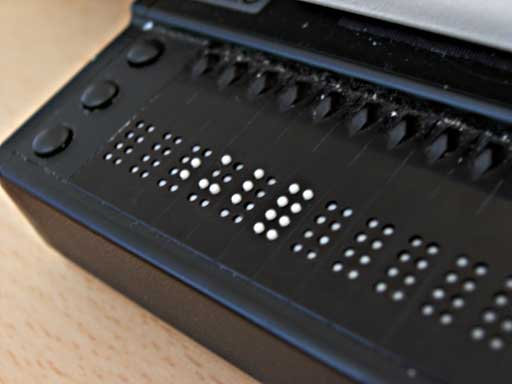
\includegraphics[scale=0.5]{Refreshable_Braille_display.jpg}
  \caption{Tauler braille (imatge presa de l'entrada \emph{Refreshable Braille Display} de la Wikipedia en anglés)}
\end{figure}

Però no només les persones amb discapacitats visuals poden tenir
problemes; qui llig un document ho pot estar fent a través d'una
pantalla de text (no gràfica) o menuda (com la d'un telèfon mòbil), o
a través d'una connexió molt lenta a la xarxa, o pot estar en una
situació en la qual els seus ulls estiguen ocupats (per exemple, quan
condueix un vehicle). La presentació de documents en aquests mitjans
té problemes similars.

Si l'èmfasi en el document ha estat emmagatzemat com a èmfasi i no amb
lletra negreta o cursiva, si els títols de secció estan indicats com a
tals i no perquè són paràgrafs d'una única línia en negretes grosses,
serà molt més fàcil transformar-lo per a la presentar-lo en un mitjà
no visual o en una pantalla reduïda o limitada, per exemple, usant
\emph{fulls d'estil} especialment concebuts per a la presentació
\emph{aural} (sonora), \emph{tàctil} (Braille), etc.

La separació de l'estructuració del contingut, d'una banda, i dels
mecanismes de presentació del document, d'una altra banda, facilita
l'\emph{accessibilitat} al document a través de diversos mitjans a
persones discapacitades o en situacions especials.

 
\section{Tecnologies auxiliars per a la generació de textos}


\subsection{Reconeixement automàtic de la parla}
\label{ss:recparla}
\com{Cal explicar millor: vocabulari obert/tancat, facilitat relativa del
reconeixement independent del parlant i dependent del parlant, etc.}

El \emph{reconeixement automàtic de la parla} (RAP) es pot definir com
la producció de textos informatitzats ---en \emph{temps real}, és a
dir, tan instantàniament com siga possible--- a partir de la veu
humana (vegeu \citealt{samuelson-brown96b}). El RAP de propòsit
general està encara molt lluny de ser perfecte, i, de fet, és encara
un camp de recerca actiu, encara que recentment s'ha incorporat
bastant satisfactòriament en dispositius com ara telèfons mòbils.\footnote{Per exemple, els dispositius amb sistema operatiu Android permeten fer recerques per veu}  En
canvi, el RAP per a un propòsit específic (per exemple, la consulta
telefònica d'horaris de trens o de les condicions del trànsit) està
molt més avançat. La major part de la inversió de la comunitat
internacional en RAP és, per raons òbvies, sobre l'anglés.

El RAP genera text a partir de la veu recollida a través d'un micròfon
utilitzant una dispositiu de captura de  per a digitalitzar-la i després un
sistema de reconeixement automàtic de la veu (\emph{automatic
  speech recognition}) per a detectar fonemes, síl·labes o paraules
completes (depén del sistema concret) i traduir-les posteriorment
a un text informatitzat.  Hi ha sistemes de reconeixement {\em
  independents del parlant} i sistemes \emph{dependents del parlant}
(els últims normalment han de ser \emph{entrenats} per la persona abans
de l'ús).  El RAP és especialment difícil per la gran variabilitat
acústica que presenten els fonemes:
\begin{itemize}
\item segons el context articulatori (per exemple, no és igual el so del
fonema palatal representat pel dígraf \emph{ig}
en ``passeig curt'' ---sord--- que en ``passeig allargat''
---sonor---);
\item segons el parlant (cada persona té uns organs fonadors de forma
  diferent ---acústicament diferents---
  i processos de producció de la parla diferents ---per exemple, n'hi
  ha qui parla més a poc a poc i qui parla molt de pressa---);
\item segons el dialecte del parlant (per exemple, els valencians fem
  africades les \emph{j} que en català central són palatals fricatives
  sonores).
\item segons l'estat emocional del parlant, etc.
\end{itemize}
És un fet ben establert que, per a superar aquestes dificultats, els
humans fem un ús molt intensiu dels coneixements lingüístics que tenim
sobre l'idioma que estem escoltant i del context comunicatiu: així, si
sentim dir ``\emph{percà nom} passes l'\emph{antre xoc} de
\emph{craus}?'' a un amic quan veiem que no pot obrir el cotxe, entenem
perfectament què ens vol dir;\footnote{\emph{Per què no em passes
    l'altre joc de claus?}} o si sentim dir en veu alta ``mu han dim
moltis baltes'' és molt probable que entenguem clarament ``m'ho han
dit moltes voltes'' a pesar dels canvis fonètics, ja que
inconscientment busquem la interpretació correcta més propera al que
hem sentit (en el context concret en què es diu la
frase).\footnote{Considereu aquest doblet anglés clàssic sobre el
  tema: \emph{people can easily recognize speech} no és molt diferent
  de {\em people can easily wreck a nice beach}; un altre doblet el
  formen les expressions \emph{sax and violins on TV} i la més
  versemblant \emph{sex and violence on TV}} Els resultats de la RAP
són especialment dependents de les particularitats lingüístiques de la
llengua involucrada i l'èxit depén de l'existència d'un bon
\emph{model de llengua} ---ràpid i concís, és a dir, computacionalment
eficient--- que simule la part no contextual de la comprensió humana i
permeta obtenir el text més probable en un idioma determinat a partir
del text en brut produït pel sistema de RAP. La major part dels
sistemes usen vocabularis grans i models estadístics.


\subsection{Reconeixement automàtic de textos escrits}
\label{ss:recautcar}

El \emph{reconeixement automàtic de textos escrits} (RATE) es pot definir
  com la producció de textos informatitzats a partir de textos
  manuscrits o tipografiats. En el cas de textos tipografiats la
  tasca és molt més senzilla; en el cas de manuscrits, la complexitat
  és comparable a la del reconeixement de la parla.
  
  El RATE genera un text informatitzat a partir d'un document imprés,
  usant un escàner (o \emph{scanner}) i càmera i un programa de
  reconeixement òptic (tam\-bé se'n diu {\em automàtic}) de caràcters
  (OCR, \emph{optical character recognition}).  Primerament, el
  document imprés és llegit (escanejat o escandit) usant l'escàner o
  la càmera, i se'n genera un fitxer que en conté la imatge digital
  (per exemple, una graella molt fina de quadrats blancs i negres).
  Després, el programa d'OCR llig la pàgina, descobreix on són els
  paràgrafs, les línies i, finalment, els caràcters concrets, i els
  transforma en un text informatitzat (normalment bastant imperfecte,
  especialment si és manuscrit).  Com en el cas del reconeixement de
  la parla, és crucial l'ús d'informació sobre l'idioma concret
  (diccionaris, estadística sobre les seqüencies de lletres) per a
  corregir els errors de l'OCR.  Per exemple, si un programa de
  lectura automàtica de textos produeix per error el text ``4ixò 6s
  uua mcrda'' no cal dir què hi llegim sense massa problemes, malgrat
  els errors en tots els mots; això és gràcies als nostres
  coneixements sobre les seqüències de lletres comunes en català.

\section{Qüestions i exercicis}
\begin{enumerate}
\item Com es diuen les combinacions especials de caràcters ASCII
  de l'estil de ``{\tt <B>}'' o ``{\tt </B>}'' que s'usen per a
  indicar tipus de lletra, grandàries de lletra, formats, etc., en
  algunes codificacions?
\begin{enumerate}
\item Marques
\item Esquemes
\item Carpetes
\end{enumerate}
\item 
   Per a validar un document XML necessitem{\ldots}
   
\begin{enumerate}
\item {\ldots} un altre document XML, aquest últim amb les
   marques sense contingut.
\item {\ldots} un full d'estil.
\item {\ldots} una definició de tipus de document.
\end{enumerate}

\item 
   Com s'indica en una DTD que l'element \verb|teixit| conté
   opcionalment els elements \verb|grandaria| 
   i \verb|color|
   en aquest ordre?
   
\begin{enumerate}
\item \verb|<!MARK teixit grandaria, color #OPTIONAL>|
\item \verb|<!MARK teixit (grandaria?,color?)>|
\item \verb|<!ELEMENT teixit (grandaria?,color?)>|
\end{enumerate}

\item 
Un document XML és \emph{vàlid}{\ldots}

\begin{enumerate}
\item {\ldots} si només usa els noms d'elements definits a la DTD; la resta de
les directrius de la DTD només serveixen per fer documents \emph{ben formats}.
\item {\ldots} si només usa les marques vàlides dels documents HTML.
\item {\ldots} si segueix les regles de la DTD quan inclou un element
dins d'un altre i, a més, no inclou cap element no definit a la DTD.
\end{enumerate}
\item 
Un text informatitzat es caracteritza principalment {\ldots} 

\begin{enumerate}
\item  {\ldots}pel seu format, d'una banda, i pel joc de caràcters
amb què està codificat, d'altra.
\item  {\ldots} per la versió del sistema operatiu i el processador de
textos amb què ha estat escrit.
\item  {\ldots}pel full d'estil que indica els aspectes estètics de la
seua presentació.
\end{enumerate}
\item Què fa que el següent fragment de XML estiga \emph{mal
   format}?
   \begin{center}\verb%<tit int=hi>Zjuknim agarnow</tit>%\end{center}
   
\begin{enumerate}
\item Entre \verb%tit% i \verb%>% no pot haver-hi res.
\item L'etiqueta \verb%tit% no és vàlida en XML; hauria de
      ser \verb%title%.
\item Si hi ha algun atribut, el valor ha d'anar entre cometes.
\end{enumerate}
\item 
   Si en una DTD trobem les regles 
   \verb%<!ELEMENT taula (capçalera?,fila+)>%, 
   \verb%<!ELEMENT fila (casella*)>% i 
   \verb%<!ELEMENT casella (#PCDATA|taula)*>% quina de les tres situacions
   següents és vàlida d'acord amb aquesta DTD?
   
\begin{enumerate}
\item 
      \verb%<taula></taula>%
      
\item 
      \verb%<taula><fila><casella>zz<taula><fila></fila></taula>zz%

      \verb%</casella><fila></taula>%
      
\item 
      \verb%<taula><fila><casella>zz</casella><casella>ww% 

      \verb%</casella></fila></taula>%
      
\end{enumerate}
\item Què indica el fragment
   \verb%encoding="%\ldots\verb%"% en la primera línia 
   (\verb%<?xml%\ldots\verb%?>%) d'un document XML?
   
\begin{enumerate}
\item La versió de XML.
\item On és la DTD necessària per a validar-lo.
\item Quin és el joc de caràcters que usa el document XML.
\end{enumerate}
\item Quants octets (\emph{bytes}) ocupa el segment de
   XML següent: \begin{center}\verb%<qq>ww</qq>%\end{center}
   
\begin{enumerate}
\item 11 com a mínim, depenent de la codificació.
\item 11, independentment de la codificació.
\item 4 exactament.
\end{enumerate}
\item Quan les marques de format només especifiquen el
   \emph{contingut} d'un document (identificant les parts i
   l'estructura de cada una), com s'assigna una \emph{presentació}
   determinada al document?
   
\begin{enumerate}
\item Amb un o més fulls d'estil.
\item Amb una codificació de caràcters (p.e., Unicode o ISO-8859-1).
\item No s'hi pot assignar presentació.
\end{enumerate}
\item Què es conserva d'ASCII en els sistemes de codificació de
   caràcters més avançats com Unicode, UTF-8, ISO-8859-1, etc.?
   
\begin{enumerate}
\item Els caràcters i els seus números de codi.
\item Els caràcters, però amb números de codi diferents.
\item No en queda res. S'ha reorganitzat tota la codificació.
\end{enumerate}
\item Som a Eslovàquia, on s'usa la codificació de caràcters 
   ISO-8859-2. Des d'Alacant, ens envien un document de text pla,
   escrit en codificació ISO-8859-1 i l'obrim com si fóra
   ISO-8859-2. Què passa? 
   
\begin{enumerate}
\item No veiem bé cap lletra: tot són símbols estranys i inintel·ligibles.
\item Veiem bé totes
   les lletres excepte les accentuades, les que porten dièresi, la
   \emph{ñ} o la \emph{ç}: en el seu lloc apareixen altres símbols
   o lletres típiques de les llengües d'Europa de l'Est.
\item Veiem bé totes
   les lletres excepte les accentuades, les que porten dièresi, la
   \emph{ñ} o la \emph{ç}: en el seu lloc apareixen les versions
   sense accent, la \emph{n} o la \emph{c}.
\end{enumerate}
\item Què és RTF?
   
\begin{enumerate}
\item Un esquema avançat de codificació de caràcters.
\item Un format obert d'intercanvi de memòries de traducció.
\item Un format obert per a intercanviar documents de text entre
      processadors de textos.
\end{enumerate}
\item Un document HTML té un enllaç amb el text ``Més informació''
   i amb URI de destinació
   \verb%http://www.detalls-e.com/mes.html%. Com és aquest
   enllaç en HTML?
   
\begin{enumerate}
\item \verb%<a href="http://www.detalls-e.com/mes.html">Més informació</a>%
\item \verb%<a href="Més informació">http://www.detalls-e.com/mes.html</a>%
\item \verb%<a htxt="Més informació" href="http://www.detalls-e.com/mes.html">%
\end{enumerate}
\item On va el títol d'un document HTML (el que es mostra en la
   \emph{barra} del navegador)?
   
\begin{enumerate}
\item En un element \verb%title% dins de \verb%head%
\item En un element \verb%title% dins de \verb%body%
\item En un element \verb%h1% dins de \verb%head%
\end{enumerate}
\item Volem digitalitzar automàticament textos impresos en paper
   que estan escrits en una llengua occidental que usa caràcters de
   l'alfabet llatí i usen tipus de lletra comuns (com ara Times,
   Courier, Arial, Helvetica, etc.). Ajuda conéixer en quina llengua
   estan escrits?
   
\begin{enumerate}
\item No, perquè la forma de les lletres no depén de la llengua,
      ja que s'usen tipus de lletra comuns.
\item No, perquè totes les llengües occidentals que usen l'alfabet
      llatí es poden codificar amb el joc de caràcters ISO-8859-15.
\item Sí, perquè cada llengua usa els caràcters de manera
      diferent per a formar paraules.
\end{enumerate}
\item Imaginem una al·locució (un segment de veu humana) en espanyol
   que pot tenir (entre d'altres) les interpretacions ``millones de
   oros'' i ``millones de euros''. Clarament, la primera és menys
   comuna que la segona. Com pot fer un sistema de reconeixement
   automàtic de parla per a elegir la segona?
   
\begin{enumerate}
\item Fent una anàlisi semàntica profunda de la frase.
\item No pot, perquè és impossible que comprenga l'espanyol parlat.
\item Usant estadístiques de aparició conjunta de paraules
      en espanyol.
\end{enumerate}

\item 
   Si els caràcters d'un text estan codificats usant el joc Latin-1
   (ISO-8859-1), quins codis tenen les lletres de la \verb|A| a
   la \verb|Z|?
   
\begin{enumerate}
\item Depén del format del text (HTML, etc.)
\item Els mateixos que en la codificació ASCII
\item Els que tenien en la codificació ASCII més 128.
\end{enumerate}

\item En un sistema de reconeixement automàtic de la parla, com es
  fa per a elegir entre \emph{efectiu} en frases com ``en efectiu''
  o ``treball efectiu'' o \emph{afectiu} en ``desenvolupament
  afectiu'' o ``àmbit afectiu''? (recordeu que en català oriental
  aquests mots es pronuncien idènticament)
  
\begin{enumerate}
\item D'acord amb la categoria lèxica del mot anterior
\item Usant la semàntica dels mots
\item Usant un model estadístic de grups de dos mots en català
\end{enumerate}

\item 
   Quants octets (\emph{bytes}) ocupa com a mínim el següent fitxer HTML?
   \begin{center}
   \verb|<html><body><p>Text.</p></body></html>|
   \end{center}
   
\begin{enumerate}
\item 11
\item 38
\item 76
\end{enumerate}

\item En la codificació ANSI ISO-8859-1, tots els caràcters
   accentuats  de l'espanyol o del català tenen codis{\ldots}
   
\begin{enumerate}
\item {\ldots}entre 0 i 127.
\item {\ldots}entre 128 i 255.
\item {\ldots}més grans que 256.
\end{enumerate}
\item Un text ANSI ISO-8859-1 té 1000 caràcters justos (comptant
   els espais en blanc i els salts de línia). Quants octets
   (\emph{bytes}) ocupa?
   
\begin{enumerate}
\item 1000 exactament, 1 per caràcter
\item 2000 exactament, 2 per caràcter
\item entre 1000 i 2000, entre 1 octet i 2 octets per caràcter
\end{enumerate}
\item En XML, si s'obri un element amb la marca
   \verb|<frase>|, amb quina marca es tanca?
   
\begin{enumerate}
\item Amb \verb|</frase>|
\item Amb \verb|<frase>|
\item Automàticament quan s'obri qualsevol altre element.
\end{enumerate}
\item   
   Si en un document XML trobem la situació
   \begin{center}\verb|<rec><id>Zork</id><addr>Zmeggs</addr></rec>|\end{center}   i una DTD defineix l'element \verb|rec| amb la regla
   \begin{center}\verb|<!ELEMENT rec (id,up?,addr*)>|\end{center} Pot
   ser que el document siga vàlid segons la DTD?
   
\begin{enumerate}
\item Depén de com siga d'estricte el programa validador
\item No, perquè aquesta situació no és vàlida.
\item Sí, si la resta del document és vàlida.
\end{enumerate}

\item 
   Què veiem si obrim un text HTML amb un editor de textos senzill com
   el \emph{bloc de notes} o \emph{Notepad} de Windows?
   
\begin{enumerate}
\item El text HTML però sense les marques entre ``\verb|<|'' i
     ``\verb|/>|''.
\item El text HTML tal com està fet per dins, amb les marques
     entre ``\verb|<|'' i
     ``\verb|>|'' i tot.
\item Una pantalla en blanc.
\end{enumerate}
\item 
   En què es diferencien dues codificacions de caràcters ANSI diferents?
   
\begin{enumerate}
\item En els caràcters assignats als 256 codis.
\item En els caràcters assignats als codis del 0 al 127.
\item En els caràcters assignats als codis del 128 al 255.
\end{enumerate}

\item 
   XML és {\ldots}
   
\begin{enumerate}
\item {\ldots}una evolució de SGML, més complexa i rica
\item {\ldots}un conjunt concret de marques entre ``\verb|<|'' i
     ``\verb|>|'' i de regles d'inclusió dels elements que
     defineixen en altres elements.
\item {\ldots}un conjunt de directrius per a definir diferents
     llenguatges consistents en marques entre ``\verb|<|'' i
     ``\verb|>|'' i en regles d'inclusió dels elements que
     defineixen en altres elements.
\end{enumerate}
\item 
   Si en una DTD trobem la regla
   \begin{center}\verb|<!ELEMENT cv (nom,any?,ob+)>|\end{center}
   quina de les tres situacions següents no és vàlida d'acord amb
   aquesta DTD?
   
\begin{enumerate}
\item 
      \verb|<cv><nom>Pere</nom><any>1992</any></cv>|
      
\item 
      \verb|<cv><nom>Pere</nom><ob>Escrits</ob></cv>|
      
\item 
      \verb|<cv><nom>Pere</nom><any>1992</any><ob>Crits</ob><ob>Plors</ob></cv>|
      
\end{enumerate}

\item 
   En un document HTML volem que la frase \emph{aquest document}
   siga un enllaç al document que té l'URI
   \verb|http://www.uc.za/t.html|: quina de les següents
   porcions de HTML és la correcta?
   
\begin{enumerate}
\item 
    \verb|<a url="http://www.uc.za/t.html">aquest document</a>|
   
\item 
     \verb|<a href="http://www.uc.za/t.html">aquest document</a>|
      
\item 
     \verb|<link url="http://www.uc.za/t.html">aquest document</link>|
     
\end{enumerate}

\item El fragment de document HTML
``\verb|<strong><em>link</strong></em>|'' 
té una errada. Quina n'és la causa?
\begin{enumerate}
\item El nom de les marques no és vàlid, perquè no n'indica cap informació
sobre el contingut.
\item L'ordre de les marques d'obertura i clausura no és correcte.
\item No s'ha indicat el valor de l'atribut \verb|href| de
l'element \verb|em|.
\end{enumerate}


\item 
Un text informatitzat es caracteritza principalment {\ldots} 

\begin{enumerate}
\item  {\ldots}pel seu format, d'una banda, i pel joc de caràcters
amb què està codificat, d'altra.
\item  {\ldots} per la versió del sistema operatiu i el processador de
textos amb què ha estat escrit.
\item  {\ldots}pel full d'estil que indica els aspectes estètics de la
seua presentació.
\end{enumerate}

\item La longitud mitjana d'un mot en gondavés és de 5,5 caràcters i
   l'edició electrònica de \emph{Gundhawól Vlâj} (``La Veu de
   Gondàvia''), té uns 100.000 mots diaris com a
   mitjana. Si el gondavés s'escriu en codificació ISO-8859-1, quants
   exemplars del diari es poden guardar en un CD-ROM?
   
\begin{enumerate}
\item Més de dos anys.
\item Un exemplar només.
\item Un mes aproximadament.
\end{enumerate}



% < QT4

\item 
   Com s'indica en una DTD que l'element \verb|<fitxa>| conté
   obligatòriament els camps \verb|<nom>| i
   \verb|<tel>| i, opcionalment, el camp \verb|<email>|?
   
\begin{enumerate}
\item \verb|<!ELEMENT fitxa (nom,tel,email?)>|
\item \verb|<!ELEMENT fitxa (nom,tel,email+)>|
\item \verb|<!ATTLIST fitxa nom CDATA #required tel CDATA #required email CDATA>|
\end{enumerate}

\item En un sistema de reconeixement automàtic dels textos escrits,
  si un mot és reconegut com a un d'aquests quatre:
  \verb|eorren|, \verb|eorrcn|, \verb|corren| o
  \verb|corrcn|, quina és la millor estratègia per a triar-ne
  una sense usar un diccionari de català (o d'espanyol)?
  
\begin{enumerate}
\item No n'hi ha, cal un diccionari.
\item Usant regles o un model estadístic que indiquen quins
  grups de dues i tres lletres estan permesos o són més freqüents en
  català (espanyol)
\item Usant regles que diuen quina lletra és més freqüent en la
  llengua corresponent.
\end{enumerate}


\item En XHTML (o HTML) hi ha elements buits (sense contingut). 
Digues en quina d'aquestes tres opcions els dos elements són buits.
\begin{enumerate}
\item \texttt{h1} i \texttt{meta}.
\item \texttt{meta} i \texttt{img}.
\texttt{meta} i \texttt{head}.
\end{enumerate}

\item En XML, què vol dir \texttt{<mang/>}? 
  \begin{enumerate}
  \item No vol dir res, perquè no hi ha cap element que es diga \texttt{mang}.
  \item El mateix que \texttt{<mang></mang>}.
  \item No vol dir res, perquè hauria de ser \texttt{</mang>}.
  \end{enumerate}

\item Quin d'aquests tres elements XHTML (o HTML) no pot anar dins de l'element \texttt{body}? 

  \begin{enumerate}
  \item \texttt{meta}.
  \item \texttt{img}.
  \item \texttt{h1}.
  \end{enumerate}


\item Tenim un document XML que és vàlid d'acord amb una determinada DTD. Esborrem un element complet (per exemple \texttt{<element>text</element>}), el qual no és l'element arrel del document. Quina d'aquestes tres situacions no és possible? 
  \begin{enumerate}
  \item Que el document XML resultant no siga vàlid respecte de la DTD.
  \item Que el document XML siga vàlid respecte de la DTD.
  \item Que el document XML no siga un document XML ben format.
  \end{enumerate}

\item En HTML, podem posar un enllaç \texttt{<a href="..."}\texttt{>...</a>} dins d'un element de llista \texttt{<li>...</li>?}  
  \begin{enumerate}
  \item Sí.
  \item No, perquè el document estaria mal format.
  \item No, perquè el document no seria vàlid.
  \end{enumerate}

\item Un fitxer de text escrit en anglés conté només caràcters ASCII. L'obrim amb un editor i el guardem en format Unicode (UTF-8). Ara ocupa{\ldots} 
  \begin{enumerate}
  \item {\ldots} el doble d'espai.
  \item {\ldots} exactament el mateix espai.
  \item {\ldots} la meitat d'espai.
  \end{enumerate}

\item En un document HTML que tindrà l'URI \texttt{http://fic.ti.cia/a.html} volem que la frase \emph{aquest document} siga un enllaç a un fitxer \texttt{http://fic.ti.cia/b.html}: quina de les següents porcions d'HTML és l'única correcta de les tres?   
  \begin{enumerate}
  \item \texttt{<a href="b.html"}\texttt{>aquest document</a>} 
  \item \texttt{<link url="http://fic.ti.cia/b.html"}\texttt{>aquest document</link>}
  \item \texttt{<a url="b.html"}\texttt{>aquest document</a>}
  \end{enumerate}

\item El fragment XML \texttt{<a><b><c></c></b></a>} no és vàlid segons una de les següents regles de DTD. Segons quina?  
  \begin{enumerate}
  \item \texttt{<!ELEMENT a (b+,c?)>}
  \item \texttt{<!ELEMENT a (b+)>}
  \item \texttt{<!ELEMENT a (b,c)>}
  \end{enumerate}

\item  Assenyala el fragment d'HTML que generarà el text més gran:  
  \begin{enumerate}
  \item \texttt{<h1>Títol</h1>}
  \item \texttt{<h2>Títol</h2>}
  \item \texttt{<h3>Títol</h3>}
  \end{enumerate}

\item Com es diu el joc de caràcters estàndard universal, el que assigna un número de codi diferent i únic a cada un dels caràcters de cada una de les llengües del món?  
  \begin{enumerate}
  \item Unicode.
  \item \emph{Latin-1}.
  \item XML.
  \end{enumerate}


\end{enumerate}
\todo{Algunes de les preguntes potser no es poden respondre amb els materials del text i caldrà eliminar-les}

\section{Solucions}
\begin{enumerate}
\item (a)
\item (c)
\item (c)
\item (c)
\item (a)
\item (c)
\item (c)
\item (c)
\item (a)
\item (a)
\item (a)
\item (b)
\item (c)
\item (a)
\item (a)
\item (c)
\item (c)
\item (b)
\item (c)
\item (b)
\item (b)
\item (a)
\item (a)
\item (c)
\item (b)
\item (c)
\item (c)
\item (a)
\item (b)
\item (b)
\item (a)
\item (a)
\item (a)
\item (b)
\item (b)
\item (c)
\item (a)
\item (c)
\item (b)
\item (c)
\item (c)
\item (a)
\item (a)
% < SL4

\end{enumerate}
